\section{Evaluation}
\label{sec:results}

We now present an evaluation of \tool. In \xref{sub:accuracy}, we evaluate
\tool's effectiveness by measuring the quality of patches and related
instrumentation required. We use the test suites bundled with the library itself
to determine if \tool\ generated patches violate any test case. We also measure
how the several optimizations (as described in \xref{subsec:optimizations})
affect the patches generated by \tool. In \xref{sub:overhead}, we measure the
relative performance and resource penalties incurred with \tool. In
\xref{sub:casestudies}, we describe our experiences with some of the major bugs
from our data set.

\ignore{
\myparagraph{Data Set} We mined bug repositories of several open-source
\java-based applications and selected $30$ bugs, majority of them being rated
either major, critical or blocking. \note{All of these bugs were very
recent and reported in the libraries which are widely used across products.
Moreover these bugs were specifically occurred in \code{String} APIs which fits
our problem definition.} These bugs involved usage of $64+$ different APIs from
\java's \code{String}, \code{StringBuffer}, \code{StringBuilder}, and Apache
\code{StringUtils} and Google Guava \code{StringUtils} classes.}

\myparagraph{Data Set} We mined bug repositories of several open-source
\java-based applications and libraries, and selected $30$ most recent
\code{String}-related bugs affecting the libraries, which are widely used across
several products. All bugs except one were rated either major, critical or
blocker. These bugs involved usage of over $64$ APIs from \java's
\code{String}, \code{StringBuffer}, \code{StringBuilder}, Apache
\code{StringUtils} and Google Guava \code{StringUtils} classes.

\myparagraph{Experimental Setup} All our experiments were performed on a laptop
with $2.9$ GHz dual core Intel i$5$ CPU, $8$ GB RAM and running Microsoft
Windows $8.1$. The JDK (v$1.7$) itself was provisioned with $2$ GB heap space.
\ignore{We used JDK v$1.7$ running with $2$ GB of allocated heap space.}
% All bug reproduction was done on Eclipse Juno IDE.
We used \infoflow\ (snapshot from May 2014)
for static taint analysis, and \soot\ v$2.5.0$ for bytecode analysis and
instrumentation.

\subsection{Accuracy}
\label{sub:accuracy}

We evaluate the precision of the patch and the effectiveness of \tool\ as
described below.

\begin{mylist}

\item \textbf{Effectiveness of the patch}: A software patch is considered
effective if it does not violate any existing test case from the software's test
suite. Thus, we determined the effectiveness of \tool\ generated patches by
running them against the benchmark's existing test suites.
Table~\ref{tab:results} lists $30$ real-world bugs mined from bug repositories
of popular open-source libraries. Column $\mathcal{T}$ lists the total number
of cases in the test suite, while $\mathcal{S}_{U}$ and $\mathcal{F}_{U}$ lists
the number of successful and failed cases in unpatched version, respectively.
Columns $\mathcal{F}_{p}$ and $\mathcal{F}_{p}^{*}$ represent the count of
failed test cases without and with \tool{}'s forced patching (to address
cascaded exceptions), respectively.

We wrote a driver program to recreate the bug, and then applied \tool\ on the
library to patch it. We observed that \tool\ without any optimizations patched
$25$ of the $30$ offending bugs in our library benchmarks, an effectiveness of
over $83\%$. With forced patching enabled to overcome cascaded exceptions arising
from \code{String} operations, \tool\ successfully patches all but two
benchmarks, thereby raising its effectiveness to over $93\%$. Note that even the
force patched versions of \code{Commons CLI2.x} and \code{Eclipse AJ Weaver}
fail test cases. We observed that in both cases the benchmarks throw a
non-\code{String} related \textit{cascaded} exception that \tool\ could not patch,
thereby resulting in failed test scenarios. A \emph{cascaded exception} is an
exception which is thrown as a response to another exception originating 
from some other program point.

\item \textbf{Precision of the patch}: Precision of a patch is governed by the
similarity between a \tool\ generated patch and the developer's fix for the same
bug. We define \textbf{Patch Precision Index (PPI)} as a measure of the
precision of the patch.
$$PPI = \frac{\#~Constraints_{\tool}}{\#~Constraints_{Developer}}$$
% * \frac{\#~LOC_{Developer}}{\#~LOC_{\tool}} *
% \frac{Output_{\tool}}{Output_{Developer}}$$

Specifically, PPI compares the similarities in constraints in \tool's patch
against the developer's version, thereby considering the core logic to construct
an effective patch. \tool\ analyzes and registers the constraints which are
related to only \code{String} objects. By doing so, we ensure that the value of
PPI is \emph{influenced} only by \code{String} objects. If \tool's patch has
fewer constraints than the developer's fix, the PPI will be lesser. Thus, a
higher value of PPI, \ie\ closer to $1$, is preferred. PPI values greater than
$1$ mean that \tool\ generates many more constraints than that of in the
developer's fix, while low values of PPI suggest that \tool\ may have missed out
on several constraints. PPI can be computed automatically, since \tool\ already
generates a list of constraints (in the form of bytecodes), and static program
analysis of the developer's patch can provide the same.
%\note{Some grammatical issue. Please fix.}

Table~\ref{tab:results} lists the PPI for the benchmarks in our set. We note
that PPI is \textgreater\ $0.7$ for over $73\%$ of the benchmarks. This high PPI
across several benchmarks indicates two things: (i) the conditional statements involved
in the developer's bug fix includes a high number of \code{String} operations,
and (ii) \tool\ correctly matches and fixes errors in several of these
\code{String} operations. PPI for the remainder of the benchmarks was observed
to be lower, \ie\ \textless\ $0.7$. On manual inspection of the concerned bugs,
we noted that the constraints in the specific conditional statement involved several
other data types other than \code{String}. Since \tool\ operates only over
\code{String} objects, the effective PPI reduces. On manual inspection of the
offending bytecodes, we observed that \tool\ generated constraints on
\code{String} conditionals were very similar to the developer's fix, thereby
confirming \tool's high precision in generating patches.

Note that taint analysis only works when sources and sinks are defined.
Since our library benchmarks have no notion of sources or sinks, \tool's
bytecode analysis of the libraries did not involve the taint analysis phase.
However, even without taint analysis, \tool's patches were of high quality, as
demonstrated by the high PPI.

\begin{table}[t]
\centering
\caption{Precision results for taint analysis.}
\scriptsize
\begin{tabular}{|l|r|r|r|}
\hline
\multicolumn{1}{|c|}{\textbf{Application}} &
\multicolumn{1}{c|}{\textbf{KLOC}} &
\multicolumn{1}{c|}{\textbf{Total paths}} &
\multicolumn{1}{c|}{\textbf{Tainted paths}}\\

\hline
\code{Checkstyle}& $58.0$ & $1977$ & $88$\\
\code{Jazzy Core}& $4.9$ & $270$ & $26$\\
\code{JEdit}& $4.3$ & $185$ & $22$\\

\hline
\end{tabular}

\label{tab:taintAnalysis}
\end{table}

\item \textbf{Precision of taint analysis}: \tool\ leverages off-the-shelf
tools (\infoflow) to perform the taint analysis. We measure precision of our
choice of tool by measuring the number of statements in the analyzed code that
are deemed unsafe to patch. Since we could not measure the precision of our
taint analysis on the library benchmarks (as discussed earlier), we select $3$
diverse applications and apply \tool\ in its entirety to obtain a measure of the
precision of the taint analysis. Specifically, for each application we provided
a set of sources, sinks and taint propagators to \infoflow, which listed the
total number of tainted paths, \ie\ paths from a sensitive source to a sink and
thus must not be patched. Table~\ref{tab:taintAnalysis} lists the results. We
observe that the total number of tainted paths is less than $12\%$ across the
applications.

\myparagraph{Threats to validity} Note that \tool\ is dependent on \infoflow\
for achieving precision about the points of instrumentation. However,
\infoflow\ currently has a major limitation---it does not support taint
analysis for multi-threaded programs. Moreover, since it is still under active
development, we observed that when applied to certain applications, \infoflow\
consumed inordinate amounts of memory and crashed. Thus, \tool's precision is
limited by the accuracy of its dependencies. 

\item \textbf{Already handled exceptions}: \tool\ analyzes the call graph to
determine if a potential runtime exception throwing statement is handled higher
up in the call chain or in the same method. In such cases \tool\ must abort the
patching effort considering that the exception is caught with exact exception
type or its base type. This is required else patching will disrupt the normal
control flow of the program.

We measure the extent of this optimization, which prevents disruption of the
control flow using the \textbf{Flow Consistency Index (FCI)} that is calculated
as $FCI = n$, where $n$ is the number of exceptions in the application that
must be ignored \tool\ for forced patching of the bug. Note that $FCI \ge 0$,
and a lower value of $FCI$ is desirable. We observe that patching four bugs
required \tool\ to ignore at most one exception; rest required no changes.

\item \textbf{Cascaded exceptions}: A cascaded exception arises if the
\tool-generated patch creates objects that when used as inputs to other \java\
APIs result in further exceptions. \tool\ is prone to cascading exceptions
because of the limitation of its intra-procedural analysis and a simple
constraint evaluation mechanism. However, \tool's constraint solver is pluggable
and a more sophisticated third party solvers can easily be integrated.
Specifically, cascaded exceptions may arise if the patch generates \code{String}
objects that represent a malformed string. Further, if we keep the optimization
in \xref{subsubsec:minimizePatchInstrumentation}, then cascaded failures may
occur even for subsequent \code{String} APIs handling the malformed
string following the point of patching. If the optimization is turned
off, \tool\ will automatically patch all relevant \code{String} APIs and thus
handle all cascaded failures involving malformed \code{String} objects.
We observe that two benchmarks throw cascaded exceptions even after being
repaired. The cascading was one level deep and triggered exception in another
non-String code (and thus unpatched), which caused the application to crash.

\end{mylist}

%already given at implementation section
\ignore{Detailed evaluation for each of the bugs in our data set is available at
\url{https://github.com/aritradhar/CLOTHO}.}

\begin{figure*}[t]
\centering
\begin{tabular}{ccc}
\subfloat[Variation in call graph analysis time with size of call
graph.\label{fig:perf:callgraph}]
{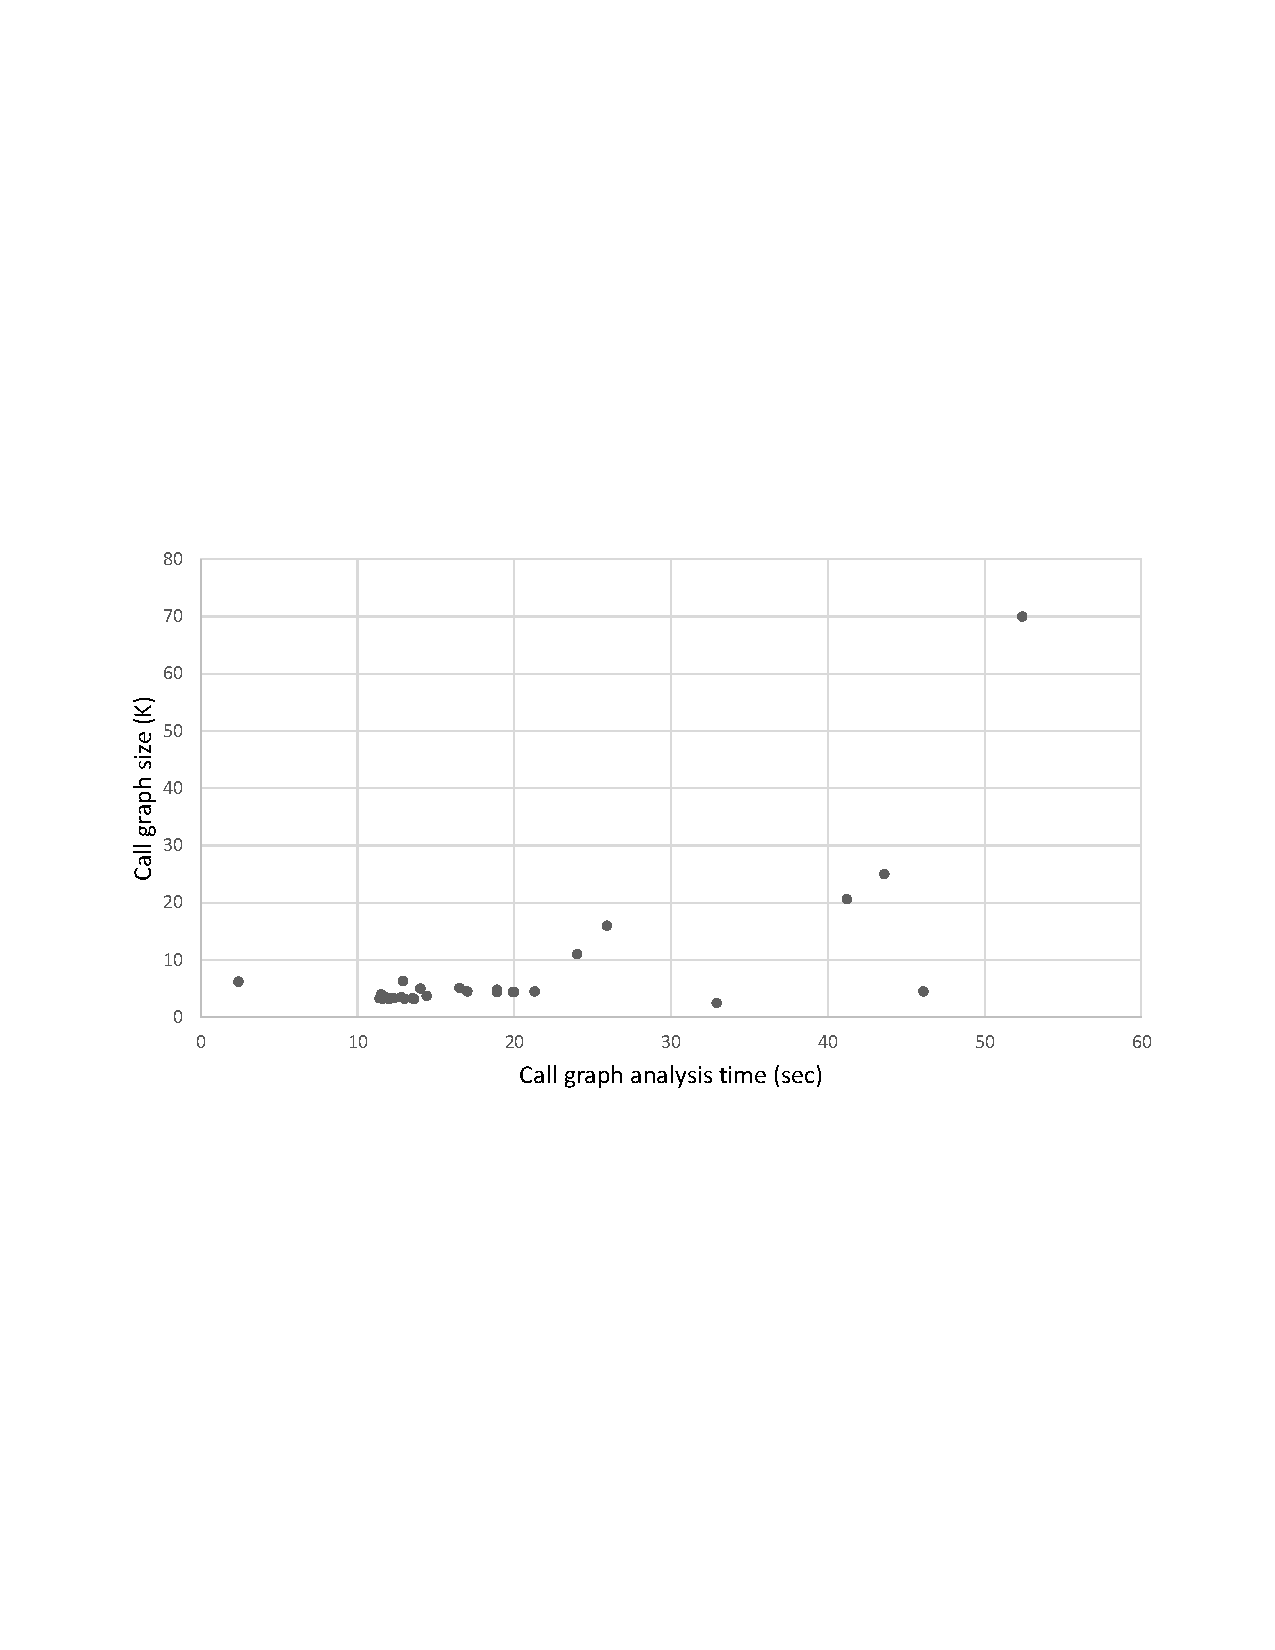
\includegraphics[width=.3\linewidth]{images/CgSizeVsTime.pdf}}
\hfill
&
\subfloat[Variation in static constraint analysis time with number of
constraints.\label{fig:perf:constraints}]
{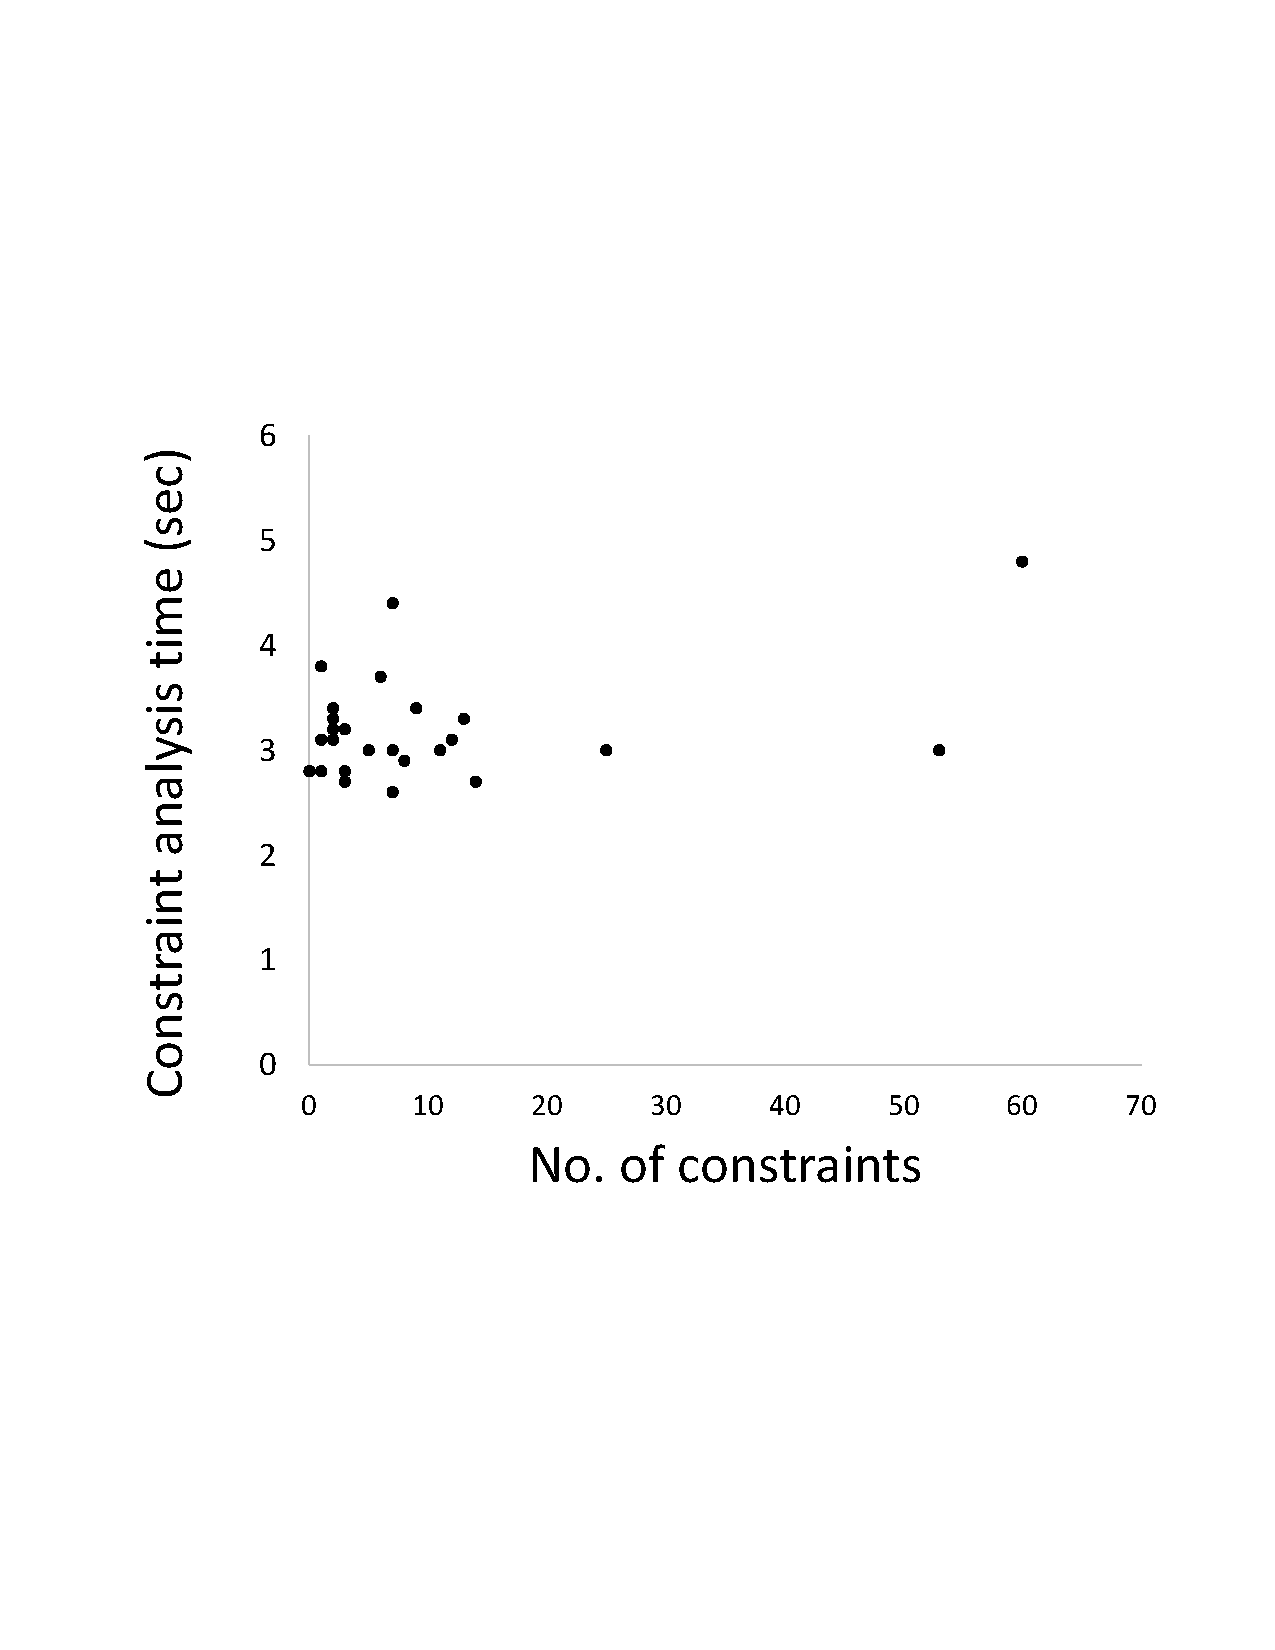
\includegraphics[width=.3\linewidth]{images/ConstraintsVsTime.pdf}
}
\hfill
&
\subfloat[Variation in instrumentation time with \code{Units} to be
instrumented.\label{fig:perf:units}]
{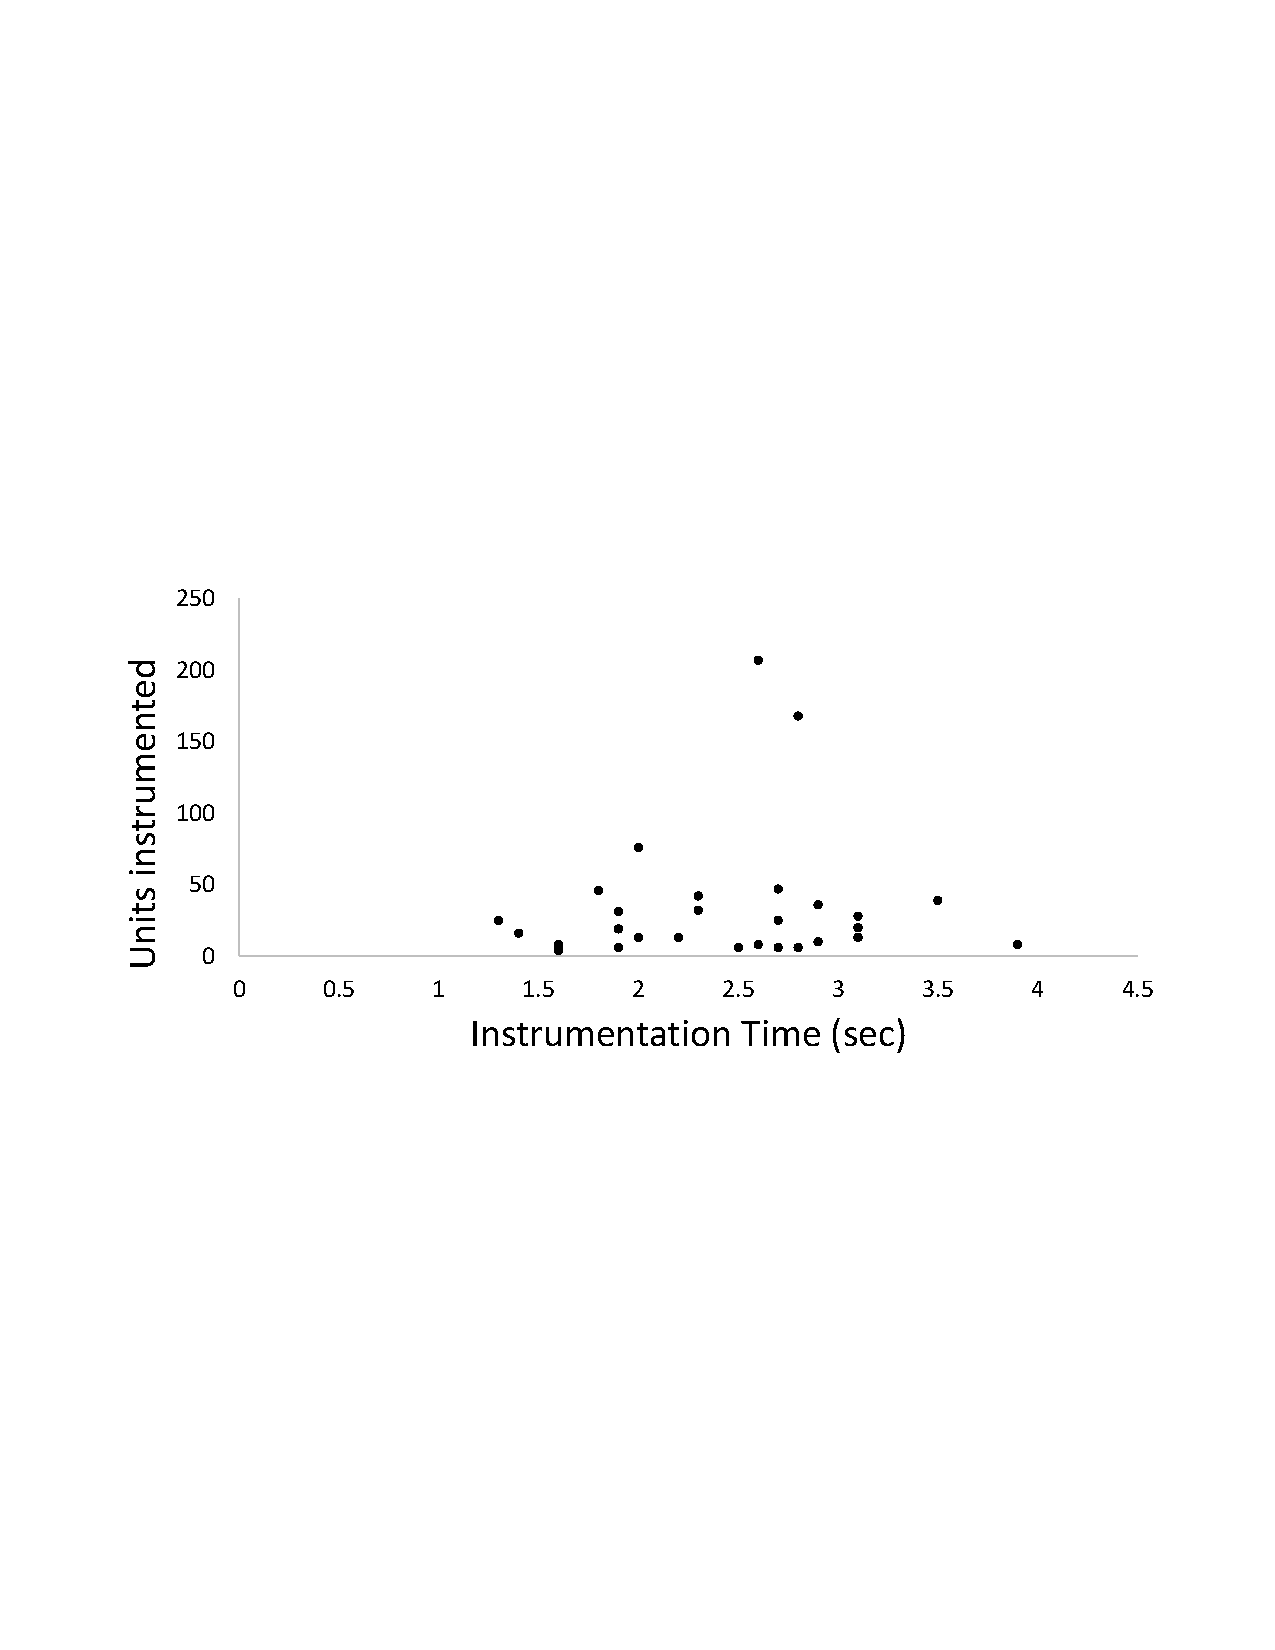
\includegraphics[width=.3\linewidth]{images/InstrumentationVsTime.pdf}}
\hfill
\\
\end{tabular}
\caption{\tool\ evaluation.}
\end{figure*}

\subsection{Overhead}
\label{sub:overhead}

We measure the overhead of \tool\ across different metrics identified below.

\begin{mylist}

 \item \textbf{Execution overhead}: We randomly selected and patched $5$
libraries (Apache Tapestry, Apache Wicket, Eclipse AspectJ Weaver, Hive and
Nutch) from Table~\ref{tab:results} to determine the execution overhead of the
patched class files. We observed that \tool\ reports an average overhead of
$\sim$$2.32\mu$s per call across the $5$ benchmarks for $50K$ runs of the
patched functionality in both the developer's version and \tool's patched
library. The maximum absolute overhead was observed for Hive at $\sim$$3.96\mu$s
per call. The above overhead is imperceptible at human response time scales.

 \item \textbf{Call graph}: The size of the call graph directly governs the time
and memory consumption for \tool. Figure~\ref{fig:perf:callgraph} shows the
results for the benchmarks analyzed from our data set. The overall analysis
time was under a minute for all the benchmarks. We observed that even for a call
graph of $\sim$$70K$ nodes (for \code{Wicket}), \tool\ required just $52.4$s
and $210$MB memory.

 \item \textbf{Constraint set}: \tool\ performs an exhaustive multi-pass
analysis to gather and evaluate the set of constraints for generating patches. A
higher number of constraints and their complexity increases the duration of
\tool's analysis. Figure~\ref{fig:perf:constraints} compares the time required
for static constraint collection and evaluation with an increasing number of
constraints for the benchmarks used in our data set. We observe that across
all the benchmarks used, \tool\ required at most $\sim$$5$s for collecting and
evaluating the constraints.

\item \textbf{Instrumentation overhead}: \tool\ performs bytecode
instrumentation for actual patching. Figure~\ref{fig:perf:units} shows the
variation in instrumentation time with increasing number of \code{Units} to be
patched. We observe that even without optimization discussed in
\xref{subsec:optimizations}, \tool\ takes under $4$s to instrument all
\code{Units} across all benchmarks. We believe that this time would be even
less with the optimizations enabled, which significantly decrease the number of
\code{Units} to be instrumented, and is evident in Table~\ref{tab:results} where
column $\mathcal{IC}_{WO}$ is much less than $\mathcal{IC}_{NO}$.

\end{mylist}

\subsection{Case studies}
\label{sub:casestudies}

We now report on experiences gained when using \tool\ to patch several of the
bugs reported in Table~\ref{tab:results}.

\begin{mylist}

 \item The bug~\cite{ARIES1204} as reported in the repository for Apache Aries
cited String related issues. However, our investigation showed that the bug was
actually in the ASM framework that was invoked by Aries, not in the Aries
framework as originally reported. Thus, we patched the particular ASM methods
containing the bugs, and retested it with the Aries framework to ensure
conformance.

 \item The bug in Commons Math~\cite{MATH198} had a bug related to incorrect
formatting of the input string. However, it threw a completely irrelevant
exception (\code{IndexOutOfBound}) instead of the \code{NumberFormatException},
which contains the information of the malformed string. The \tool-generated
patch fixes the undesirable behavior.

 \item The bug in OfBiz~\cite{OFBIZ4237} throws a custom shutdown exception,
when in fact it should throw a \code{StringIndexOutOfBoundsException} due to a
\code{substring} invocation with incorrect bounds. This ultimately causes the
library to throw some high priority exception and ultimately crash if not handed
properly by the application. The patched version of the library catches the
correct exception.

 \item The code to trigger bugs in some libraries, including Apache Commons
Compress, Commons Lang, Commons Math and Ofbiz, each had string operations
wrapped in \code{try-catch} block that were handled by \code{Exception} class,
\ie\ the base type of all exceptions. However, \tool\ checks for already
handled runtime exceptions during its call graph analysis, and thus did not
patch the bugs. We turned off the call graph analysis module to force \tool\ to
generate the relevant patch for the bug.

 \item We also noticed several instances where the developer code does not
follow proper programming practices regarding exception handling. For example,
the SOAP bug~\cite{SOAP130} was reported for a faulty \code{substring} call that
threw a \code{StringIndexOutOfBoundsException}. The entire method was wrapped in
a \code{try-catch} that included the faulty substring call along with other
servlet operations. However, the \code{catch} block handled the generic
\code{Exception}, which is the base class of all exceptions. Thus, both servlet
exceptions or \code{IndexOutOfBoundException} from the \code{substring} call
were handled in a generic fashion. \tool's patched library ensures that
exceptions originating from the \code{substring} call are handled properly.

\end{mylist}